%!TEX root =  bgo.tex
% please do not delete or change the first line (needed by Csaba's editor)

Notation: Capital letters will denote random variables.
For $p\le q$ integers, \todoc{natural numbers?}
 we use the notation $a_{p:q}$ to denote
 the sequence $(a_p,a_{p+1}, \dots, a_{q})$.


\begin{figure}
\begin{center}
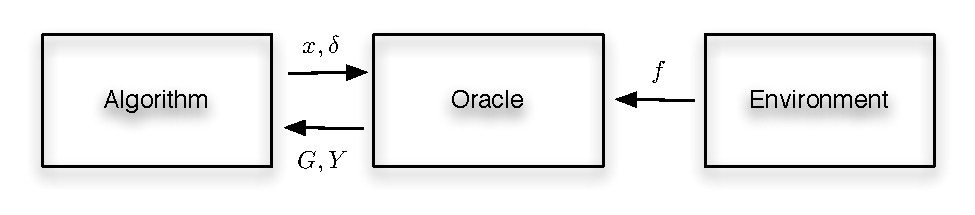
\includegraphics[width=0.45\textwidth]{figs/oracle}
\end{center}
\caption{The Interaction of the algorithms with the gradient estimation oracle and the environment. For more information, see the text.}
\label{fig:oracle}
\end{figure}

In this paper we consider convex optimization in a novel setting, both for online learning and optimization. 
%More specifically, we consider both an online learning setting and an optimization setting.
In the online setting, the environment chooses a sequence of loss functions $f_1,\dots,f_n$ belonging to a set $\cF$ of convex functions over a common, non-empty convex closed domain $\cK\subset \R^d$. 
In the optimization setting, a single fixed loss function $f\in \cF$ is chosen.
As usual, the algorithms choose a sequence of points $X_1,\dots,X_n\in \cK$ in a sequential way. 
The novelty of our setting is that the algorithm, upon selecting point $X_t$, receives 
a noisy and potentially biased estimate $G_t\in \R^d$ 
of the gradient of the loss function $f$ 
(more generally, an estimate of a subgradient of $f$ in case $f$ is non-differentiable at $X_t$). 
To control the bias and the variance the algorithm can choose a \emph{tolerance parameter} $\delta_t>0$ 
(in particular, we allow the algorithms to choose the tolerance parameter sequentially). 
A smaller $\delta_t$ results in a smaller ``bias'' (for the precise meaning of bias, we will consider two definitions below), while typically with a smaller $\delta_t$ the ``variance'' of the gradient estimate increases.
The algorithm also receives a point $Y_t\in \cK$, which is guaranteed to be in the $\delta_t$-vicinity of $X_t$. 
While this point is not relevant in the optimization setting, in the online learning setting, 
the algorithm suffers a loss at $Y_t$.
As usual, the goal in the online setting is to keep the expected \emph{regret}, 
	$R_n =\EE{ \sum_{t=1}^n f_t(Y_t)} - \inf_{x\in \cK} \sum_{t=1}^n f_t(x)$,
small.
In the optimization setting, the algorithm is also required to select a point $\hat{X}_n\in \cK$ once
the $n$th round is over (in both settings, $n$ is given to the algorithms)
and the algorithm's performance is quantified using the \emph{optimization error}, 
$\Delta_n = \EE{f(\hat{X}_n)} - \inf_{x\in \cK} f(x) $.

The main novelty of the model is that the information flow between the algorithm and the environment is controlled by the gradient estimation oracle. As we shall see, numerous existing approaches to online learning and optimization based on noisy pointwise information fit this framework. 

In what follows, the functions $c_1,c_2:[0,\infty)\to [0,\infty)$ will be assumed to be continuous, 
monotonously increasing (resp., decreasing) with 
$\lim_{\delta\to  0} c_1(\delta)=0$ and $\lim_{\delta\to 0} c_2(\delta)=+\infty$.
Typical choices for $c_1,c_2$ are $c_1(\delta) = C_1 \delta^p$, $c_2(\delta) = C_2\delta^{-q}$ with $p,q>0$.
We define two classes of oracles. The relationship between these oracles will be studied in \cref{sec:orrel}.
\begin{definition}[$(c_1,c_2)$ Type-I  oracle]
\label{def:oracle1}
We say that $\gamma$ is a  $(c_1,c_2)$ Type-I oracle, if for any function $f\in \cF$,
$x\in \cK,\delta>0$, $\gamma$ returns $G\in \R^d$ and  $Y\in \cK$ random elements such that:
\begin{enumerate}
\item $\norm{x-Y}\le \delta$ almost surely (a.s.);
\item $\norm{ \EE{G}  - \nabla f(x)  }_* \le c_1(\delta) $; and
\item $\EE{\norm{ G -  \EE{G} }_*^2} \le c_2(\delta)$.
\end{enumerate}
\end{definition}
The second type of oracle considered is as follows:
\begin{definition}[$(c_1,c_2)$ Type-II  oracle]
\label{def:oracle2}
We say that $\gamma$ is a  $(c_1,c_2)$ Type-II oracle, if for any function $f\in \cF$,
$x\in \cK,\delta>0$, $\gamma$ returns $G\in \R^d$ and  $Y\in \cK$ random elements such that:
\begin{enumerate}
\item $\norm{x-Y}\le \delta$ a.s.;
\item There exists $\tilde{f} \in \cF$ such that  
$\norm{\tilde{f}- f}_\infty \le c_1(\delta)$  and
$\EE{G}  = \nabla \tilde{f}(x)$ (bias);
\item $\EE{\norm{ G -  \EE{G} }_*^2} \le c_2(\delta)$ (variance).
\end{enumerate}
\end{definition}
An alternative to the bias condition for Type-II oracles, which will also be considered later, is to replace the condition $\norm{\tilde{f}-f}_\infty \le c_1(\delta)$ with \todoc{This requires $f$ to be differentiable.. Or define using subgradients?}
\begin{align}
\label{eq:oracle2alt}
\norm{\nabla \tilde{f}- \nabla f}_\infty \le c_1(\delta).
\end{align}
Note that our definition allows the same oracle $\gamma$ to respond to the same inputs $(x,\delta,f)$ with a differently constructed pair (e.g., to have memory), 
though most often the oracles constructed in practice 
will map the triples $(x,\delta,f)$ to a gradient estimate-point pair using a stochastic mapping.
\todoc{In fact, I am not sure which definition we should use. So things might change here.}
There are several examples of oracles satisfying these definitions; see \cref{sec:ex}.
We will denote the set of Type-I (Type-II) oracles satisfying the $(c_1,c_2)$-requirements given a function $f\in \cF$ by $\Gamma_1(f,c_1,c_2)$ (resp., $\Gamma_2(f,c_1,c_2)$). 

In this paper we will study the minimax regret in the online setting, while we study the minimax error in the optimization setting (sometimes, also called as the ``simple regret'').
Both are defined with respect to a class of loss functions $\cF$, and the bias/variance control functions $c_1,c_2$.
The minimax expected regret for $(\cF,c_1,c_2)$ with Type-I oracles is
\begin{align}
\label{eq:minimaxregdef}
\MoveEqLeft
R_n^*(\cF,c_1,c_2) 
= \inf_{\cA} \sup_{f_{1:n}\in \cF^n} 
	\sup_{\substack{\gamma_t \in \Gamma_1(f_t,c_1,c_2)\\1\le t \le n}} R_n^{\cA}(f_{1:n},\gamma_{1:n})
%\\
%\MoveEqLeft
%= \inf_{\cA} \sup_{f_{1:n}\in \cF} 
%	\sup_{\substack{\gamma_t \in \Gamma_1(f_t,c_1,c_2)\\1\le t \le n}} 
%\EE{ \sum_{t=1}^n f_t(Y_t) }  
%%%%%%& \qquad \qquad \qquad \qquad \qquad 
%-\inf_{x\in \cK} \sum_{t=1}^n f_t(x)\,,\\
\end{align}
where $\cA$ ranges through all algorithms that interact with the $f_{1:n}= (f_1,\dots,f_n)$ loss sequence
as described earlier
through the oracles $\gamma_{1:n}$,
and we use $R_n^{\cA}(f_{1:n},\gamma_{1:n})$ the expected regret of $\cA$ against $(f_{1:n},\gamma_{1:n})$.
The minimax regret for Type-II (and other similar) oracles is defined analogously (in what follows we only define these quantities for Type-I oracles, as the extension to other types of oracles is immediate).

In the optimization setting, the minimax error is defined through
\begin{align}
\label{eq:minimaxerrdef}
\Delta_n^*(\cF,c_1,c_2)
= \inf_{\cA} \sup_{f \in \cF} \sup_{\gamma\in \Gamma_1(f,c_1,c_2)}  \Delta_n^{\cA}(f,\gamma)\,,
% \EE{ f(\hat{X}_n) } - \inf_{x\in \cK}  f(x)\,,
\end{align}
where, again, $\cA$ ranges through all algorithms that interact with the loss $f$ through $\gamma$ and 
$\Delta_n^{\cA}(f,\gamma)$ is the optimization error that $\cA$ suffers 
after $n$ rounds of interaction with $f$ through $\gamma$ as described earlier.
%$\hat{X}_n$ is the point returned by $\cA$ after $n$ rounds of interaction which work as described earlier.

